%!TEX root = ../../book_ML.tex
\chapter{Phân cụm $K$-means}
\index{phân cụm $K$-means -- $K$-means clustering}
\label{cha:kmeans}
\section{Giới thiệu}
Trong Chương~\ref{cha:linear_regression} và, \ref{cha:knn}, chúng ta đã làm quen
các thuật toán học có giám sát. Trong chương này, một thuật toán đơn giản của
học không giám sát sẽ được trình bày. Thuật toán này có tên là \textit{phân cụm
$K$-means} (\textit{$K$-means clustering}).

Trong phân cụm $K$-means, ta không biết nhãn của từng
điểm dữ liệu. Mục đích là làm thể nào để phân dữ liệu thành các cụm (cluster)
khác nhau sao cho dữ liệu trong cùng một cụm có những tính chất giống nhau.

\textbf{Ví dụ:} Một công ty muốn tạo ra một chính sách ưu đãi cho những nhóm
khách hàng khác nhau dựa trên sự tương tác giữa mỗi khách hàng với công ty đó
(số năm là khách hàng, số tiền khách hàng đã chi trả cho công ty, độ tuổi, giới
tính, thành phố, nghề nghiệp,...). Giả sử công ty có dữ liệu của khách hàng
nhưng phân cụm. Phân cụm $K$-means là một thuật toán có thể giúp thực hiện
công việc này. Sau khi phân cụm, nhân viên công ty có thể quyết định mỗi
nhóm tương ứng với nhóm khách hàng nào. Phần việc cuối cùng này cần sự can thiệp
của con người, nhưng lượng công việc đã được rút gọn đi đáng kể.

\index{cụm -- cluster}

Một nhóm/cụm có thể được định nghĩa là tập hợp các điểm có
vector đặc trưng gần nhau. Việc tính toán khoảng cách có thể phụ thuộc vào từng loại dữ liệu, trong đó khoảng cách Euclid được sử dụng phổ biến nhất. Trong chương này, các tính toán được thực hiện dựa trên khoảng cách Euclid. Tuy nhiên, quy trình thực hiện thuật toán có thể được áp dụng cho các loại khoảng cách khác. 

% ******************************************************************************
\begin{figure}[t]
    % caption on side     
    \floatbox[{\capbeside\thisfloatsetup{capbesideposition={right,top},capbesidewidth=6cm}}]{figure}[\FBwidth]
    {\caption{ 
    Ví dụ với ba cụm dữ liệu trong không gian hai chiều. 
    }
    \label{fig:4_1}}
    { % figure here
    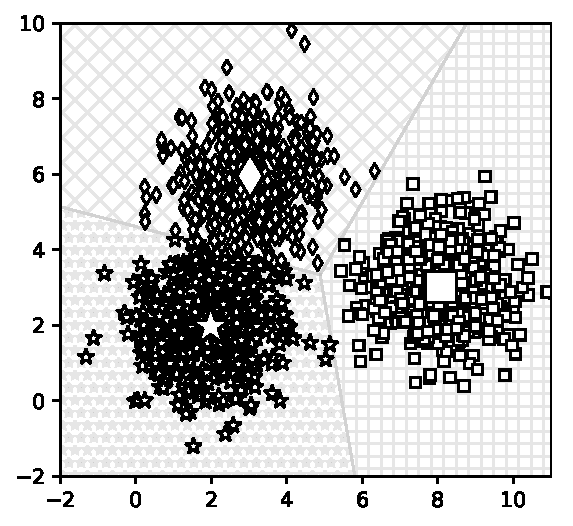
\includegraphics[width=.5\textwidth]{ebookML_src/src/kmeans/ex_5notitle.pdf}
    % 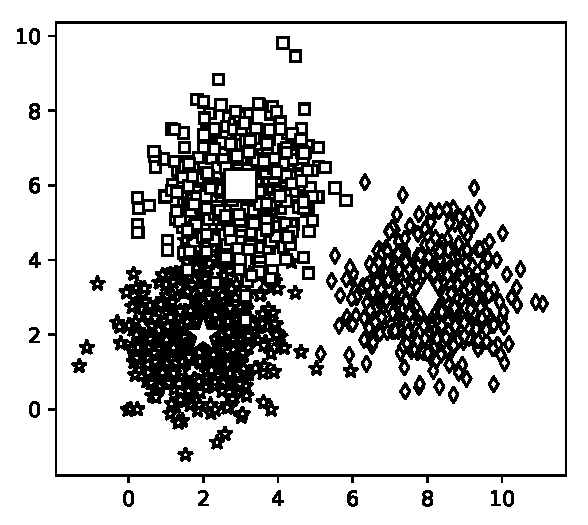
\includegraphics[width=.5\textwidth]{ebookML_src/src/kmeans/data.pdf}
    }
\end{figure}
% ******************************************************************************
\index{phân cụm $K$-means -- $K$-means clustering!tâm cụm -- centroid}

Hình~\ref{fig:4_1} là một ví dụ về dữ liệu được phân vào ba cụm. Giả sử mỗi cụm
có một điểm đại diện được gọi là \textit{tâm cụm}, được minh hoạ bởi các điểm
màu trắng lớn. Mỗi điểm thuộc vào cụm có tâm gần nó nhất. Tới đây, chúng ta có
một bài toán thú vị: {Trên vùng biển hình chữ nhật có ba đảo hình thoi, hình
vuông và sao năm cánh lớn màu trắng như Hình~\ref{fig:4_1}. Một điểm trên biển
được gọi là thuộc lãnh hải của một đảo nếu nó nằm gần đảo này hơn so với hai đảo
còn lại. Hãy xác định ranh giới lãnh hải giữa các đảo.}

% \index{hyperpolygon -- siêu đa diện}
Cũng trên Hình~\ref{fig:4_1}, các vùng với nền khác nhau biểu thị lãnh hải của
mỗi đảo. Có thể thấy rằng đường phân định giữa các lãnh hải có dạng đường
thẳng. Chính xác hơn, chúng là đường trung trực của các cặp đảo gần nhau. Vì
vậy, lãnh hải của một đảo sẽ là một hình đa giác. Cách phân chia dựa trên khoảng
cách tới điểm gần nhất này trong toán học được gọi là Voronoi
diagram\footnote{\textit{Vonoroi diagram -- Wikipedia}
(\url{https://goo.gl/xReCW8}).}. Trong không gian ba chiều, lấy ví dụ là các
hành tinh, \textit{lãnh không} của mỗi hành tinh sẽ là một đa diện. Trong không
gian nhiều chiều hơn, chúng ta sẽ có những \textit{siêu đa diện}.

% Quay lại với bài toán phân cụm và cụ thể là thuật toán phân cụm $K$-means,
% chúng ta cùng thảo luận cơ sở toán học, cách xây dựng và tối ưu hàm mất mát của
% nó.


% chúng ta cần một chút phân tích toán học trước khi đi tới phần
% \href{http://machinelearningcoban.com#tom-tat-thuat-toan}{tóm tắt thuật toán} ở
% phần dưới. Nếu bạn không muốn đọc quá nhiều về toán, bạn có thể bỏ qua phần này.
% (\textit{Tốt nhất là đừng bỏ qua, bạn sẽ tiếc đấy}).

\section{Phân tích toán học }

Mục đích cuối cùng của thuật toán phân cụm $K$-means là từ dữ liệu đầu vào và số
lượng cụm cần tìm, hãy xác định tâm mỗi cụm và phân các điểm dữ liệu vào cụm
tương ứng. Giả sử thêm rằng mỗi điểm dữ liệu chỉ thuộc đúng một cụm.


% \subsection{Một số ký hiệu toán học}
Giả sử $N$ điểm dữ liệu trong tập huấn luyện được ghép lại thành ma trận $ \mathbf{X} =
[\mathbf{x}_1, \mathbf{x}_2, \dots,
\mathbf{x}_N] \in \mathbb{R}^{d \times N}$ và $K < N$ là số cụm được xác định trước. Ta cần tìm các tâm cụm $ \mathbf{m}_1, \mathbf{m}_2,
\dots, \mathbf{m}_K \in \mathbb{R}^{d \times 1}$ và nhãn của mỗi điểm dữ liệu.
Ở đây, mỗi cụm được đại diển bởi một nhãn, thường là một số tự nhiên từ 1
đến $K$. Nhắc lại rằng các điểm dữ liệu trong bài toán phân cụm $K$-means ban
đầu không có nhãn cụ thể. 

\index{mã hoá one-hot -- one-hot coding}
Với mỗi điểm dữ liệu $\bx_i$, ta cần tìm nhãn $y_i = k$ của nó, ở đây $k\in
\{1, 2, \dots, K\}$. Nhãn của một điểm cũng thường được biểu diễn dưới dạng một
vector hàng $K$ phần tử $\by_i \in \R^{1\times K}$, trong đó tất cả các phần tử
của $\by_i$ bằng 0 trừ phần tử ở vị trí thứ $k$ bằng 1. Cách biểu diễn này còn
được gọi là mã hoá \textit{one-hot}. Cụ thể, $y_{ij} = 0,~\forall j \neq k,
y_{ik} = 1$. Khi {chồng} các vector $\by_i$ lên nhau, ta được một ma trận nhãn
$\bY \in \R^{N\times K}$. Nhắc lại rằng $y_{ij}$ là phần tử hàng thứ $i$, cột
thứ $j$ của ma trận $\bY$, và cũng là phần tử thứ $j$ của vector $\by_i$. Ví dụ,
nếu một điểm dữ liệu có vector nhãn là $[1,0,0,\dots,0]$ thì nó thuộc vào cụm
thứ nhất, là $[0,1,0,\dots,0]$ thì nó thuộc vào cụm thứ hai,... Điều kiện của
$\mathbf{y}_i $ có thể viết dưới dạng toán học:
\begin{equation}
\label{eqn:4_1} y_{ij} \in \{0, 1\},~\forall i, j;~~~ \sum_{j = 1}^K y_{ij} = 1, ~\forall i
\end{equation}
\subsection{Hàm mất mát và bài toán tối ưu}

Gọi $\mathbf{m}_k \in \R^{d}$ là tâm của cụm thứ $k$. Giả sử một điểm dữ liệu
$\mathbf{x}_i $ được phân vào cụm $k$. Vector sai số nếu thay $\bx_i$ bằng
$\bm_k$ là $(\mathbf{x}_i - \mathbf{m}_k) $. Ta muốn vector sai số này gần với
vector không, tức $\bx_i$ gần với $\bm_k$. Việc này có thể được thực hiện thông
qua việc tối thiểu bình phương khoảng cách Euclid $\|\mathbf{x}_i -
\mathbf{m}_k\|_2^2$. Hơn nữa, vì $\mathbf{x}_i $ được phân vào cụm $k$ nên $y_{ik} = 1, y_{ij} = 0, ~\forall j \neq k $. Khi đó, biểu thức khoảng cách Euclid có thể được viết lại thành
\begin{equation}
  \|\mathbf{x}_i - \mathbf{m}_k\|_2^2 = y_{ik}\|\mathbf{x}_i -
  \mathbf{m}_k\|_2^2 =  \sum_{j=1}^K y_{ij}\|\mathbf{x}_i - \mathbf{m}_j\|_2^2
\end{equation}
Như vậy, sai số trung bình cho toàn bộ dữ liệu sẽ là:
\begin{equation}
  \mathcal{L}(\mathbf{Y}, \mathbf{M}) = \frac{1}{N}\sum_{i=1}^N\sum_{j=1}^K
  y_{ij} \|\mathbf{x}_i - \mathbf{m}_j\|_2^2
\end{equation}
Trong đó $\mathbf{M} = [\mathbf{m}_1, \mathbf{m}_2, \dots, \mathbf{m}_K] \in
\R^{d\times K} $ là ma trận tạo bởi $K$ tâm cụm. Hàm mất mát trong bài toán
phân cụm $K$-means là $\mathcal{L}(\mathbf{Y}, \mathbf{M})$ với
ràng buộc như được nêu trong~\eqref{eqn:4_1}.
Để tìm các tâm cụm và cụm tương ứng của mỗi điểm dữ liệu, ta cần giải bài toán tối ưu có ràng buộc
\begin{equation}
\label{eqn:4_2}
\begin{aligned}
\mathbf{Y}, \mathbf{M} &= \argmin_{\mathbf{Y}, \mathbf{M}}
\frac{1}{N}\sum_{i=1}^N\sum_{j=1}^K y_{ij} \|\mathbf{x}_i -
\mathbf{m}_j\|_2^2\\
\text{thoả mãn:} &~ y_{ij} \in \{0, 1\},~\forall i, j;~~~ \sum_{j = 1}^K
y_{ij} = 1,~\forall i
\end{aligned}
\end{equation}

\subsection{Thuật toán tối ưu hàm mất mát}
Bài toán~\eqref{eqn:4_2} là một bài toán khó tìm {điểm tối ưu} vì có
thêm các điều kiện ràng buộc. \textit{Bài toán này thuộc loại mix-integer
programming (điều kiện biến là số nguyên) - là loại rất khó tìm nghiệm tối ưu
toàn cục.} Tuy nhiên, trong một số trường hợp chúng ta vẫn có 
phương pháp để tìm nghiệm gần đúng. Một kỹ thuật đơn giản và phổ biến để
giải bài toán~\eqref{eqn:4_2} là xen kẽ giải $\mathbf{Y}$ và $\mathbf{M}$ khi
biến còn lại được cố định cho tới khi hàm mất mát hội tụ. Chúng ta sẽ lần lượt giải
quyết hai bài toán sau.

\subsubsection{Cố định $\mathbf{M} $, tìm $\mathbf{Y}$ }

\textit{Giả sử đã tìm được các tâm cụm, hãy tìm các vector nhãn để hàm mất mát
đạt giá trị nhỏ nhất.} 

Khi các tâm cụm là cố định, bài toán tìm vector nhãn cho toàn bộ dữ liệu
có thể được chia nhỏ thành bài toán tìm vector nhãn cho từng điểm dữ liệu
$\mathbf{x}_i$ như sau:
\begin{equation}
\label{eqn:4_3}
\begin{aligned}
  \mathbf{y}_i &= \argmin_{\mathbf{y}_i} \frac{1}{N} \sum_{j=1}^K
  y_{ij}\|\mathbf{x}_i -
  \mathbf{m}_j\|_2^2 \\
  \text{thoả mãn:}~ & y_{ij} \in \{0, 1\},~\forall i, j; \quad \sum_{j = 1}^K
  y_{ij} = 1,
  ~\forall i.
\end{aligned}
\end{equation}
Vì chỉ có một phần tử của vector nhãn $\mathbf{y}_i$ bằng $1$ nên bài
toán~\eqref{eqn:4_3} chính là bài toán đi tìm tâm cụm gần điểm $\bx_i$ nhất:
\begin{equation}
j = \argmin_{j} \|\mathbf{x}_i - \mathbf{m}_j\|_2^2.
\end{equation}
Vì $\|\mathbf{x}_i - \mathbf{m}_j\|_2^2$ là bình phương khoảng cách Euclid
từ điểm $\mathbf{x}_i $ tới centroid $\mathbf{m}_j $, ta có thể kết luận rằng
\textit{mỗi điểm $\mathbf{x}_i $ thuộc vào cụm có tâm gần nó nhất}. Từ đó có thể
suy ra vector nhãn của từng điểm dữ liệu.

\subsubsection{Cố định $\mathbf{Y} $, tìm $\mathbf{M}$ }

\textit{Giả sử đã biết cụm của từng điểm, hãy tìm các tâm
cụm mới để hàm mất mát đạt giá trị nhỏ nhất.}

Khi vector nhãn cho từng điểm dữ liệu đã được xác định, bài toán
tìm tâm cụm được rút gọn thành
\begin{equation}
\label{eqn:5_mj}
\mathbf{m}_j = \argmin_{\mathbf{m}_j} \frac{1}{N}\sum_{i = 1}^{N}
y_{ij}\|\mathbf{x}_i - \mathbf{m}_j \|_2^2.
\end{equation}
Để ý rằng hàm mục tiêu là một hàm liên tục và có đạo hàm xác định tại mọi điểm
$\bm_j$. Vì vậy, ta có thể tìm nghiệm bằng phương pháp giải phương trình đạo hàm
bằng không. Đặt $l(\mathbf{m}_j)$ là hàm mục tiêu bên trong dấu $\argmin$
của~\eqref{eqn:5_mj}, ta cần giải phương trình sau đây:
\begin{eqnarray}
\label{eqn:4_mj2}
\nabla_{\bm_j} l(\bm_j) =  \frac{2}{N}\sum_{i=1}^N
y_{ij}(\mathbf{m}_j - \mathbf{x}_i) = \bzero \\
\Leftrightarrow\mathbf{m}_j \sum_{i=1}^N y_{ij} = \sum_{i=1}^N y_{ij}
\mathbf{x}_i
\Leftrightarrow \mathbf{m}_j = \frac{ \sum_{i=1}^N y_{ij}
\mathbf{x}_i}{\sum_{i=1}^N y_{ij}}
\end{eqnarray}
Để ý rằng mẫu số chính là tổng {số điểm dữ liệu} trong cụm $j$, tử số là
{tổng các điểm dữ liệu} trong cụm $j$. Nói cách khác, $\mathbf{m}_j$
{là trung bình cộng (mean) của các điểm trong cụm} $j$.

Tên gọi \textit{phân cụm $K$-means} xuất phát từ đây.

\subsection{Tóm tắt thuật toán}
Tới đây, ta có thể tóm tắt thuật toán K-means cụming như sau. 
\begin{myalg}{phân cụm $K$-means}{kmeans}
    
\textbf{Đầu vào:} Ma trận dữ liệu $\mathbf{X} \in \R^{d \times N}$ và số lượng
cụm cần tìm $K < N$.

\textbf{Đầu ra:} Ma trận tâm cụm $\mathbf{M} \in \R^{d \times K}$ và ma trận
nhãn $\mathbf{Y} \in \R^{N\times K}$.

\begin{enumerate}
    \item[1.] Chọn $K$ điểm bất kỳ trong tập huấn luyện làm các tâm cụm ban đầu.

    \item[2.]  Phân mỗi điểm dữ liệu vào cụm có tâm gần nó nhất.

    \item[3.]  Nếu việc phân cụm dữ liệu vào từng cụm ở bước 2 không thay đổi
    so với vòng lặp trước nó thì dừng thuật toán.

    \item[4.]  Cập nhật tâm cụm bằng cách lấy trung bình cộng của các điểm đã được gán vào cụm đó sau bước 2.

    \item[5.]  Quay lại bước 2.
\end{enumerate}
\end{myalg}


Thuật toán này sẽ hội tụ sau một số hữu hạn vòng lặp. Thật vậy, dãy số biểu diễn giá trị của hàm mất mát sau mỗi bước là một đại
lượng không tăng và bị chặn dưới. Điều này chỉ ra rằng dãy số này phải hội tụ.
Để ý thêm nữa, số lượng cách phân cụm cho toàn bộ dữ liệu là hữu hạn (khi số
cụm $K$ là cố định) nên đến một lúc nào đó, hàm mất mát sẽ không thể thay
đổi, và chúng ta có thể dừng thuật toán tại đây.

Nếu tồn tại một cụm không chứa điểm nào, mẫu số trong~\eqref{eqn:4_mj2} sẽ
bằng không, và phép chia sẽ không thực hiện được. Vì vậy, $K$ điểm bất kỳ trong
tập huấn luyện được chọn làm các tâm cụm ban đầu ở bước 1 để đảm bảo mỗi
cụm có ít nhất một điểm. Trong quá trình huấn luyện, nếu tồn tại một cụm
không chứa điểm nào, có hai cách giải quyết. Cách thứ nhất là bỏ cụm đó
và giảm $K$ đi một. Cách thứ hai là thay tâm của cụm đó bằng một điểm
bất kỳ trong tập huấn luyện, chẳng hạn như điểm xa tâm cụm hiện tại của nó nhất.
 % (sai số xấp xỉ là lớn nhất).

\section{Ví dụ trên Python}


\subsection{Giới thiệu bài toán}
Chúng ta sẽ làm một ví dụ đơn giản. Trước hết, ta tạo tâm cụm và dữ liệu cho
từng cụm bằng cách lấy mẫu theo phân phối chuẩn có kỳ vọng là tâm của
cụm đó và ma trận hiệp phương sai là ma trận đơn vị. Ở đây, hàm
\pythoninline{cdist} trong \pythoninline{scipy.spatial.distance} được dùng để
tính khoảng cách giữa các cặp điểm trong hai tập hợp một cách hiệu
quả\footnote{việc xây dựng hàm số này không sử dụng thư viện đã được thảo luận
kỹ trong Chương~\ref{cha:knn}}.

Dữ liệu được tạo bằng cách lấy ngẫu nhiên 500 điểm cho mỗi cụm theo phân
phối chuẩn có kỳ vọng lần lượt là \pythoninline{(2, 2), (8, 3)} và
\pythoninline{(3, 6)}; ma trận hiệp phương sai giống nhau và là ma trận đơn vị.
\begin{lstlisting}[language=Python]
from __future__ import print_function 
import numpy as np 
import matplotlib.pyplot as plt
from scipy.spatial.distance import cdist
import random
np.random.seed(18)
means = [[2, 2], [8, 3], [3, 6]]
cov = [[1, 0], [0, 1]]
N = 500
X0 = np.random.multivariate_normal(means[0], cov, N)
X1 = np.random.multivariate_normal(means[1], cov, N)
X2 = np.random.multivariate_normal(means[2], cov, N)
X = np.concatenate((X0, X1, X2), axis = 0)
K = 3 # 3 clusters 
original_label = np.asarray([0]*N + [1]*N + [2]*N).T
\end{lstlisting}


% \subsection{Hiển thị dữ liệu trên đồ thị}

% Chúng ta cần một hàm \pythoninline{kmeans_display} để hiển thị dữ liệu. Sau đó
% hiển thị dữ liệu theo nhãn ban đầu.


% \begin{lstlisting}[language=Python]
% def kmeans_display(X, label):
%     K = np.amax(label) + 1
%     X0 = X[label == 0, :]
%     X1 = X[label == 1, :]
%     X2 = X[label == 2, :]

%     plt.plot(X0[:, 0], X0[:, 1], 'b^', markersize = 4, alpha = .8)
%     plt.plot(X1[:, 0], X1[:, 1], 'go', markersize = 4, alpha = .8)
%     plt.plot(X2[:, 0], X2[:, 1], 'rs', markersize = 4, alpha = .8)

%     plt.axis('equal')
%     plt.plot()
%     plt.show()

% kmeans_display(X, original_label)
% \end{lstlisting}


% % <div class="imgcap">
% % <img src ="/assets/kmeans/output_5_0.png" align = "centroid">
% % </div>
% Trong đồ thị trên, mỗi cluster tương ứng với một màu. Có thể nhận thấy rằng có
% một vài điểm màu đỏ bị lẫn sang phần cluster màu xanh.

\subsection{Các hàm số cần thiết cho phân cụm $K$-means }
Trước khi viết thuật toán chính phân cụm $K$-means, ta cần một số hàm phụ
trợ: 
\begin{enumerate}
    \item \pythoninline{kmeans_init_centroids} khởi tạo các tâm cụm.

    \item \pythoninline{kmeans_asign_labels} tìm nhãn mới cho các điểm khi
    biết các tâm cụm.

    \item \pythoninline{kmeans_update_centroids} cập nhật các tâm cụm khi
    biết nhãn của từng điểm. 

    \item \pythoninline{has_converged} kiểm tra điều kiện dừng của thuật toán.
\end{enumerate}


\begin{lstlisting}[language=Python]
def kmeans_init_centroids(X, k):
    # randomly pick k rows of X as initial centroids
    return X[np.random.choice(X.shape[0], k, replace=False)]
\end{lstlisting}

\begin{lstlisting}[language=Python]
def kmeans_assign_labels(X, centroids):
    # calculate pairwise distances btw data and centroids
    D = cdist(X, centroids)
    # return index of the closest centroid
    return np.argmin(D, axis = 1)

def has_converged(centroids, new_centroids):
    # return True if two sets of centroids are the same
    return (set([tuple(a) for a in centroids]) ==
        set([tuple(a) for a in new_centroids]))

def kmeans_update_centroids(X, labels, K):
    centroids = np.zeros((K, X.shape[1]))
    for k in range(K):
        # collect all points that are assigned to the k-th cluster
        Xk = X[labels == k, :]
        centroids[k,:] = np.mean(Xk, axis = 0) # take average 
    return centroids
\end{lstlisting}
Phần chính của phân cụm $K$-means:


\begin{lstlisting}[language=Python]
def kmeans(X, K):
    centroids = [kmeans_init_centroids(X, K)]
    labels = []
    it = 0
    while True:
        labels.append(kmeans_assign_labels(X, centroids[-1]))
        new_centroids = kmeans_update_centroids(X, labels[-1], K)
        if has_converged(centroids[-1], new_centroids):
            break
        centroids.append(new_centroids)
        it += 1
    return (centroids, labels, it)
\end{lstlisting}

Áp dụng thuật toán vừa viết vào dữ liệu ban đầu và hiển thị kết quả cuối cùng:


\begin{lstlisting}[language=Python]
(centroids, labels, it) = kmeans(X, K)
print('Centers found by our algorithm:\n', centroids[-1])
kmeans_display(X, labels[-1])
\end{lstlisting}
% \newpage 
\kq
\begin{lstlisting}
Centers found by our algorithm:
 [[ 1.9834967   1.96588127]
 [ 3.02702878  5.95686115]
 [ 8.07476866  3.01494931]]
\end{lstlisting}

% <div class="imgcap">
% <img src ="/assets/kmeans/output_11_1.png" align = "centroid">
% </div>

Hình~\ref{fig:4_example} minh hoạ thuật toán phân cụm $K$-means trên tập dữ
liệu này sau một số vòng lặp. Nhận thấy rằng tâm cụm và các vùng
\textit{lãnh thổ} của chúng thay đổi qua các vòng lặp và hội tụ chỉ sau sáu vòng
lặp. Từ kết quả này ta thấy rằng thuật toán phân cụm $K$-means làm việc
khá thành công, các tâm cụm tìm được gần với các tâm cụm ban đầu và các nhóm
dữ liệu được phân ra gần như hoàn hảo (một vài điểm gần ranh giới giữa hai
cụm hình thoi và hình sao có thể lẫn vào nhau).

% Dưới đây là hình ảnh động minh họa thuật toán qua từng vòng lặp, chúng ta thấy
% rằng thuật toán trên hội tụ rất nhanh, chỉ cần 6 vòng lặp để có được kết quả
% cuối cùng:
% <div class="imgcap">
% <img src ="/assets/kmeans/kmeans11.gif" align = "centroid">
% </div>

%%%%%%% Three subfigures with bottom caption%%%%%%%%%%%%%%
\begin{figure}[t]
    \begin{subfigure}{0.325\textwidth}
    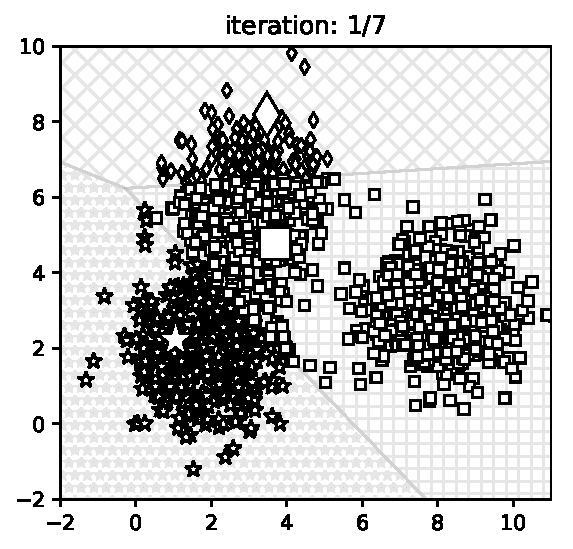
\includegraphics[width=0.99\linewidth]{ebookML_src/src/kmeans/ex_0.pdf}
    % \caption{}
    % \label{fig:subim1}
    \end{subfigure}
    \begin{subfigure}{0.325\textwidth}
    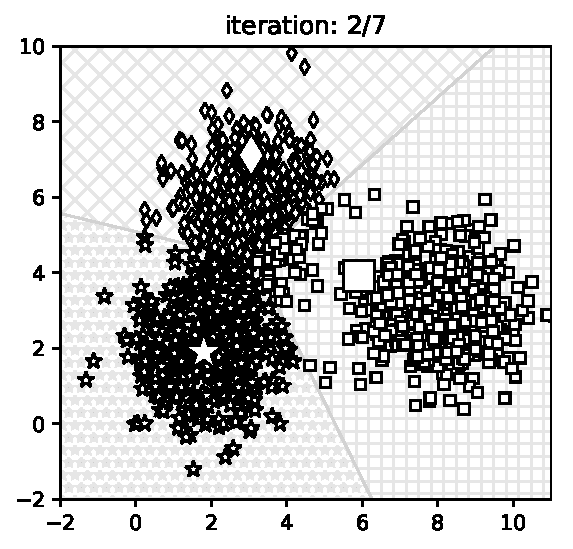
\includegraphics[width=0.99\linewidth]{ebookML_src/src/kmeans/ex_1.pdf}
    % \caption{}
    % \label{fig:subim2}
    \end{subfigure}
    \begin{subfigure}{0.325\textwidth}
    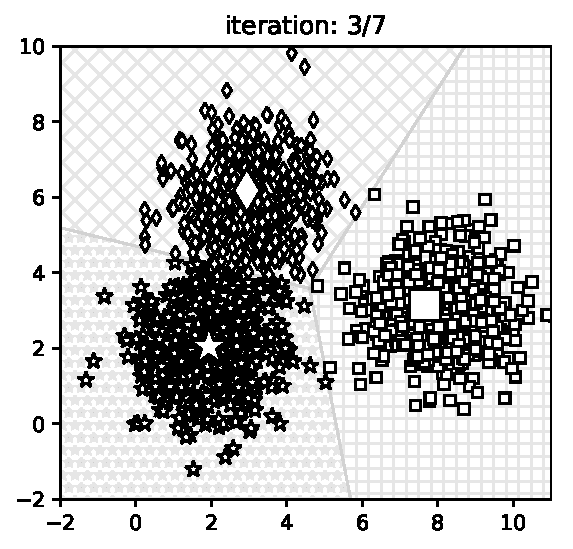
\includegraphics[width=0.99\linewidth]{ebookML_src/src/kmeans/ex_2.pdf}
    % \caption{}
    % \label{fig:subim2}
    \end{subfigure}

    \begin{subfigure}{0.325\textwidth}
    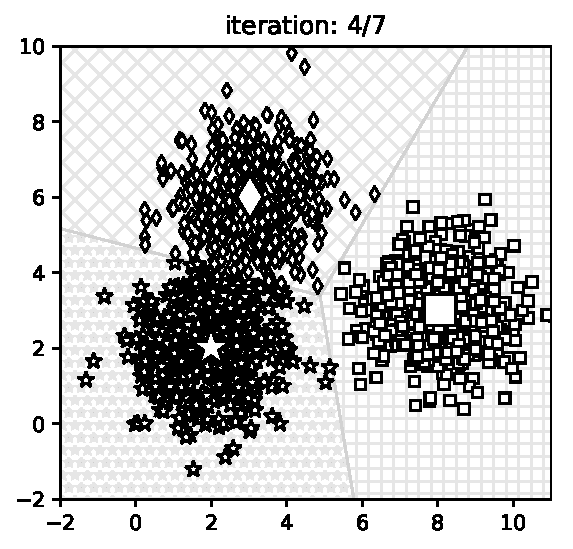
\includegraphics[width=0.99\linewidth]{ebookML_src/src/kmeans/ex_3.pdf}
    % \caption{}
    % \label{fig:subim1}
    \end{subfigure}
    \begin{subfigure}{0.325\textwidth}
    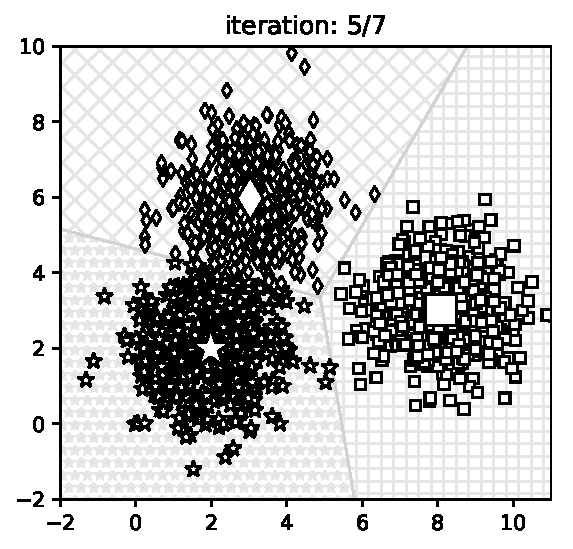
\includegraphics[width=0.99\linewidth]{ebookML_src/src/kmeans/ex_4.pdf}
    % \caption{}
    % \label{fig:subim2}
    \end{subfigure}
    \begin{subfigure}{0.325\textwidth}
    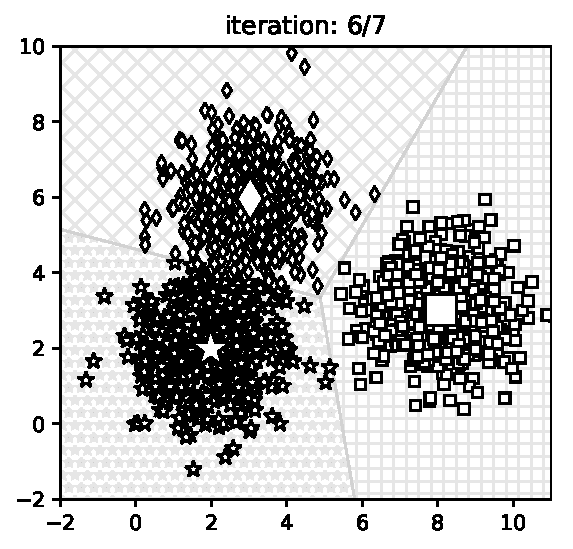
\includegraphics[width=0.99\linewidth]{ebookML_src/src/kmeans/ex_5.pdf}
    % \caption{}
    % \label{fig:subim2}
    \end{subfigure}
    \caption{
        Thuật toán phân cụm $K$-means qua các vòng lặp.     
    }
    \label{fig:4_example}
\end{figure}


% Các bạn có thể xem thêm các trang web minh họa thuật toán K-means cluster tại:


\subsection{Kết quả tìm được bằng thư viện scikit-learn}

Để kiểm tra thêm, chúng ta hãy so sánh kết quả trên với kết quả thu được bằng
cách sử dụng thư viện
\href{http://scikit-learn.org/stable/modules/generated/sklearn.cluster.KMeans.html}{\pythoninline{scikit-learn}}.

\begin{lstlisting}[language=Python]
from sklearn.cluster import KMeans
model = KMeans(n_clusters=3, random_state=0).fit(X)
print('Centers found by scikit-learn:')
print(model.cluster_centers_)
pred_label = model.predict(X)
kmeans_display(X, pred_label)
\end{lstlisting}
\kq 
\begin{lstlisting}
Centroids found by scikit-learn:
    [[ 8.0410628   3.02094748]
     [ 2.99357611  6.03605255]
     [ 1.97634981  2.01123694]]
\end{lstlisting}
Ta nhận thấy rằng các tâm cụm tìm được rất gần với kết quả kỳ vọng. 

Tiếp theo, chúng ta cùng xem xét ba ứng dụng đơn giản của phân cụm $K$-means. 

% <div class="imgcap">
% <img src ="/assets/kmeans/output_14_1.png" align = "centroid">
% </div>


% Thật may mắn (\textit{cho tôi}), hai thuật toán cho cùng một đáp số! Với cách
% thứ nhất, tôi mong muốn các bạn hiểu rõ được thuật toán K-means clustering làm
% việc như thế nào. Với cách thứ hai, tôi hy vọng các bạn biết áp dụng thư viện
% sẵn có như thế nào.



\section{Phân cụm chữ số viết tay }

\subsection{Bộ cơ sở dữ liệu MNIST }
\index{MNIST}

MNIST~\cite{lecun2010mnist} là bộ cơ sở dữ liệu lớn nhất về chữ số viết tay và
được sử dụng trong hầu hết các thuật toán phân loại hình ảnh. MNIST bao gồm hai
tập con: tập huấn luyện có 60 nghìn mẫu và tập kiểm tra có 10 nghìn mẫu. Tất cả
đều đã được gán nhãn. Hình~\ref{fig:5_mnist} hiển thị 200 mẫu được trích ra từ
MNIST.




Mỗi bức ảnh là một ảnh xám (chỉ có một kênh), có kích thước $28\times28$
điểm ảnh (tức 784 điểm ảnh). Mỗi điểm ảnh mang giá trị là một số tự nhiên từ 0
đến 255. Các điểm ảnh màu đen có giá trị bằng không, các điểm ảnh càng trắng thì có giá trị càng cao. Hình~\ref{fig:5_digit7} là một ví dụ về chữ
số 7 và giá trị các điểm ảnh của nó\footnote{Vì mục đích hiển thị ma trận điểm ảnh ở
bên phải, bức ảnh kích thước $28 \times 28$ ban đầu đã được resize về kích thước
$14 \times 14$.}.

\begin{figure}[t]
    % caption on side     
    \floatbox[{\capbeside\thisfloatsetup{capbesideposition={right,top},capbesidewidth=.2\textwidth}}]{figure}[\FBwidth]
    {\caption{ 
        200 mẫu ngẫu nhiên trong bộ cơ sở dữ liệu MNIST. 
    }
    \label{fig:5_mnist}}
    { % figure here
    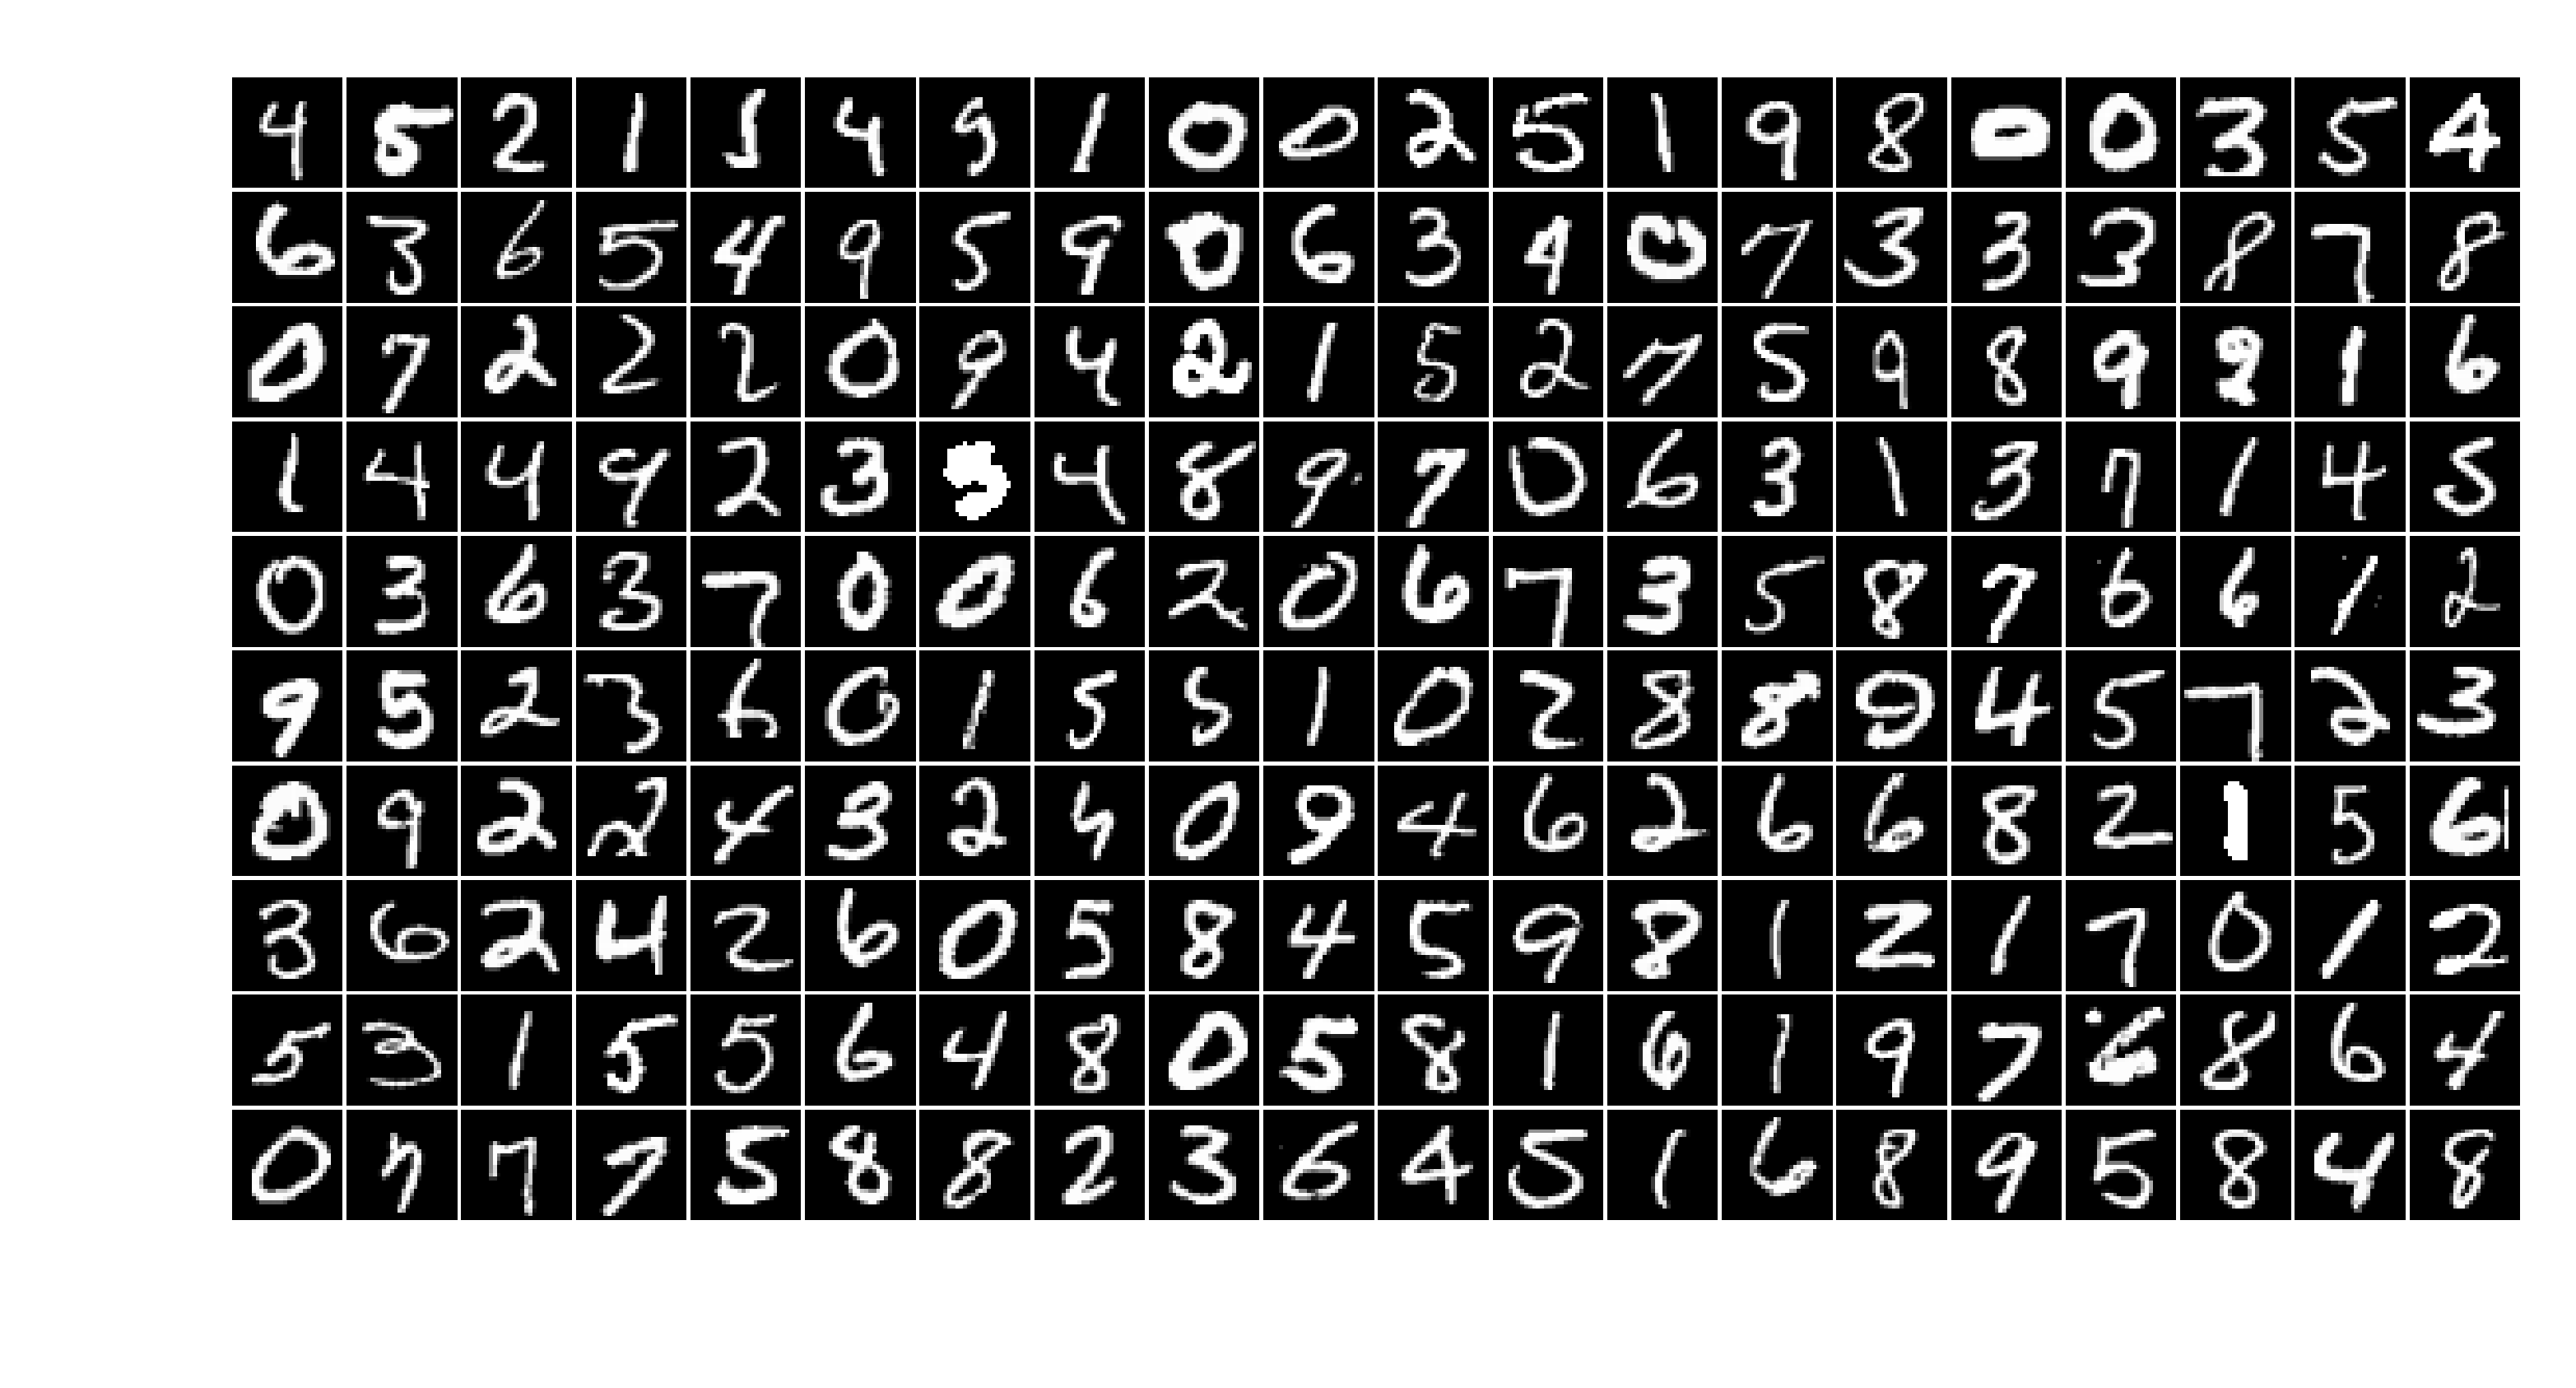
\includegraphics[width=.75\textwidth]{ebookML_src/src/kmeans/mnist_ex.png}
    }
\end{figure}
\begin{figure}[t]
    % caption on side     
    \floatbox[{\capbeside\thisfloatsetup{capbesideposition={right,top},capbesidewidth=3.5cm}}]{figure}[\FBwidth]
    {\caption{ 
    Ví dụ về chữ số 7 và giá trị các pixel của nó. 
    }
    \label{fig:5_digit7}}
    { % figure here
    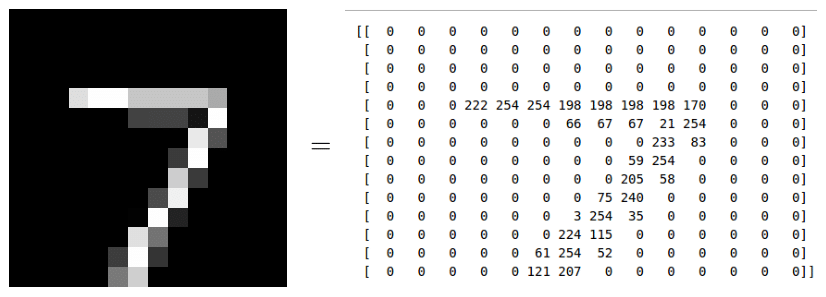
\includegraphics[width=.75\textwidth]{Chapters/03_SimpleML/4_kmeans/digit_7.png}
    }
\end{figure}


\subsection{Bài toán phân cụm giả định}
\textit{\textbf{Bài toán}}: Giả sử ta không biết nhãn của các bức ảnh, hãy phân
các bức ảnh gần giống nhau về một cụm.

Bài toán này có thể được giải quyết bằng phân cụm $K$-means. Mỗi bức ảnh có thể
được coi là một điểm dữ liệu với vector đặc trưng là vector cột 784 chiều.
Vector này nhận được bằng cách chồng các cột của ma trận điểm ảnh lên nhau.

% Trước khi áp dụng thuật toán
% \href{http://machinelearningcoban.com/2017/01/01/kmeans/}{K-means clustering},
% chúng ta cần coi mỗi bức ảnh là một điểm dữ liệu. Và vì mỗi điểm dữ liệu là 1
% vector (hàng hoặc cột) chứ không phải ma trận như số 7 ở trên, chúng ta phải làm
% thêm một bước đơn giản trung gian gọi là \textit{vectorization} (vector hóa).
% Nghĩa là, để có được 1 vector, ta có thể tách các hàng của ma trận pixel ra, sau đó
% đặt chúng cạnh nhau, và chúng ta được một vector hàng rất dài biểu diễn 1 bức
% ảnh chữ số.

% \textbf{Chú ý}: \textit{Cách làm này chỉ là cách đơn giản nhất để mô tả dữ liệu
% ảnh bằng 1 vector. Trên thực tế, người ta áp dụng rất nhiều kỹ thuật khác nhau để
% có thể tạo ra các vector đặc trưng (feature vector) giúp các thuật toán có được
% kết quả tốt hơn.}


\subsection{Làm việc trên Python}
Để tải về MNIST, chúng ta có thể dùng trực tiếp một hàm số trong scikit-learn:

\begin{lstlisting}[language=Python]
from __future__ import print_function 
import numpy as np 
from sklearn.datasets import fetch_mldata

data_dir = '../../data' # path to your data folder 
mnist = fetch_mldata('MNIST original', data_home=data_dir)
print("Shape of minst data:", mnist.data.shape)
\end{lstlisting}
\kq 
\begin{lstlisting}[language=Python]
Shape of minst data: (70000, 784)
\end{lstlisting}
\pythoninline{shape} của ma trận dữ liệu \pythoninline{mnist.data} là
\pythoninline{(70000, 784)} tức có 70000 mẫu, mỗi mẫu có kích thước 784. Chú ý
rằng trong scikit-learn, mỗi điểm dữ liệu thường được lưu dưới dạng một vector
hàng. Tiếp theo, chúng ta lấy ra ngẫu nhiên 10000 mẫu và thực hiện phân cụm $K$-means
trên tập con này:
% \newpage 
\begin{lstlisting}[language=Python]
from sklearn.cluster import KMeans
from sklearn.neighbors import NearestNeighbors
K = 10 # number of clusters 
N = 10000
X = mnist.data[np.random.choice(mnist.data.shape[0], N)]
kmeans = KMeans(n_clusters=K).fit(X)
pred_label = kmeans.predict(X)
\end{lstlisting}





Sau khi thực hiện đoạn code trên, các tâm cụm được lưu trong biến
\pythoninline{kmeans.cluster_centers_}, nhãn của mỗi điểm dữ liệu được lưu
trong biến \pythoninline{pred_label}. Hình~\ref{fig:5_random} hiển thị các tâm
cụm tìm được và 20 mẫu ngẫu nhiên được phân vào cụm tương ứng. Mỗi hàng tương
ứng với một cụm, cột đầu tiên bên trái là các tâm cụm tìm được. Ta thấy rằng các
tâm cụm đều giống với một chữ số hoặc là kết hợp của hai/ba chữ số nào đó. Ví
dụ, tâm cụm ở hàng thứ tư là sự kết hợp của các chữ số 4, 7, 9; ở hàng thứ bảy là kết
hợp của các chữ số 7, 8 và 9.





Nhận thấy rằng các bức ảnh lấy ra ngẫu nhiên từ mỗi cụm không thực sự giống
nhau. Lý do có thể vì những bức ảnh này ở xa các tâm cụm mặc dù tâm cụm đó đã là
gần nhất. Như vậy phân cụm $K$-means làm việc chưa thực sự tốt trong trường hợp
này. Tuy nhiên, chúng ta vẫn có thể khai thác một số thông tin hữu ích sau khi
thực hiện thuật toán. Thay vì chọn ngẫu nhiên các bức ảnh trong mỗi cụm, ta chọn
20 bức ảnh gần tâm của mỗi cụm nhất, vì càng gần tâm thì độ tin cậy càng cao.
Quan sát Hình~\ref{fig:5_knn}, có thể thấy dữ liệu trong mỗi hàng khá giống nhau
và giống với tâm cụm ở cột đầu tiên bên trái. Từ đây có thể rút ra một vài quan
sát thú vị:

\begin{enumerate}
    \item Có hai kiểu viết chữ số 1 -- thẳng và chéo. Phân cụm $K$-means
    nghĩ rằng đó là hai chữ số khác nhau. Điều này là dễ hiểu vì phân cụm $K$-means
    là một thuật toán học không giám sát. Nếu có sự can thiệp của
    con người, chúng có thể được nhóm lại thành một. 


    \item Ở hàng thứ chín, chữ số 4 và 9 được phân vào cùng một cụm. Sự
    thật là hai chữ số này khá giống nhau. Điều tương tự xảy ra đối với
    hàng thứ bảy với các chữ số 7, 8, 9. Phân cụm $K$-means có thể được áp dụng để tiếp tục phân nhỏ các cụm đó.

\end{enumerate}

\begin{figure}[t]
    % caption on side     
    \floatbox[{\capbeside\thisfloatsetup{capbesideposition={right,top},capbesidewidth=4cm}}]{figure}[\FBwidth]
    {\caption{ 
    Các tâm cụm (cột đầu) và 20 điểm {ngẫu nhiên} trong mỗi cụm. Các chữ số trên mỗi hàng thuộc vào cùng một cụm.
    }
    \label{fig:5_random}}
    { % figure here
    % 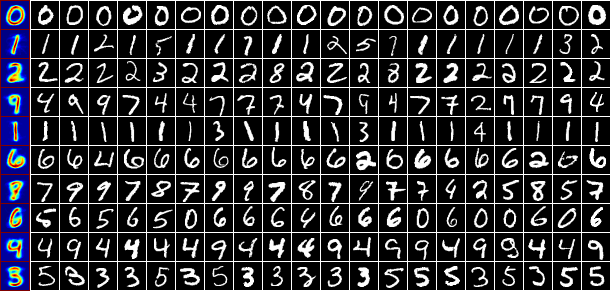
\includegraphics[width=.65\textwidth]{Chapters/03_SimpleML/4_kmeans/kmeans_random.png}
    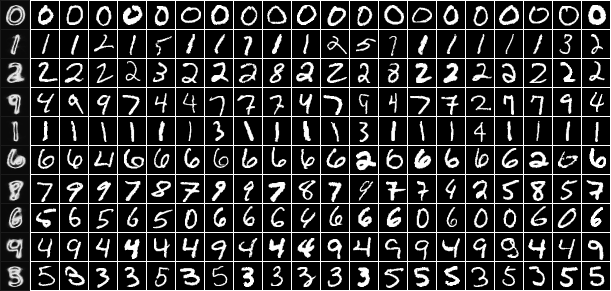
\includegraphics[width=.65\textwidth]{Chapters/03_SimpleML/4_kmeans/kmeans_random_gray.png}
    }
\end{figure}

\begin{figure}[t]
    % caption on side     
    \floatbox[{\capbeside\thisfloatsetup{capbesideposition={right,top},capbesidewidth=4cm}}]{figure}[\FBwidth]
    {\caption{ 
    Tâm và 20 điểm gần tâm nhất của mỗi cụm.
    }
    \label{fig:5_knn}}
    { % figure here
    % 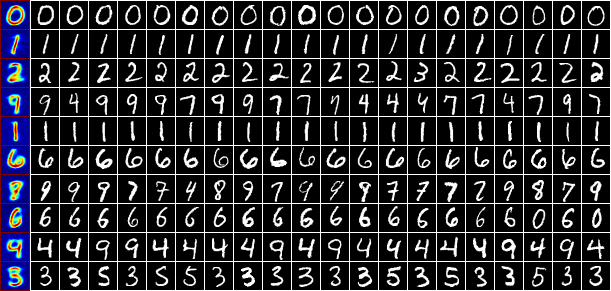
\includegraphics[width=.65\textwidth]{Chapters/03_SimpleML/4_kmeans/kmeans_knn.png}
    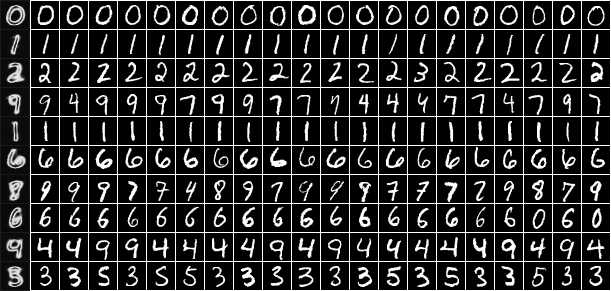
\includegraphics[width=.65\textwidth]{Chapters/03_SimpleML/4_kmeans/kmeans_knn_gray.png}
    }
\end{figure}

\index{phân cụm theo tầng -- hierarchical clustering}
Một kỹ thuật phân cụm thường được sử dụng là \textit{phân cụm theo
tầng} (\textit{hierarchical clustering}~\cite{blei2008hierarchical}). Có hai
loại phân cụm theo tầng:

\begin{itemize}
    \item \textit{Agglomerative} tức ``đi từ dưới lên''. Ban đầu ta chọn $K$ là một
    số lớn gần bằng số điểm dữ liệu. Sau khi thực hiện phân cụm $K$-means lần
    đầu, các cụm gần nhau được ghép lại thành một cụm. Khoảng cách giữa các cụm có thể được xác định bằng khoảng cách giữa các tâm cụm. Sau bước này, ta thu được một
    số lượng cụm nhỏ hơn. Tiếp tục phân cụm $K$-means với điểm khởi tạo
    là tâm của cụm lớn vừa thu được. Lặp lại quá trình này đến khi nhận
    được kết quả chấp nhận được.

    \item \textit{Divisive} tức ``đi từ trên xuống''. Ban đầu, thực hiện phân
    cụm $K$-means với $K$ nhỏ để được các cụm lớn. Sau đó tiếp tục áp dụng phân cụm $K$-means vào mỗi cụm lớn đến khi kết quả chấp nhận được.

\end{itemize}

% \newpage 
\section{Tách vật thể trong ảnh}


% \subsection{Đặt vấn đề}
Phân cụm $K$-means cũng được áp dụng vào bài toán \textit{tách vật thể trong ảnh} (\textit{object segmentation}). Cho bức ảnh như trong Hình~\ref{fig:5_girl}, hãy xây dựng một thuật toán tự động nhận diện và tách rời vùng khuôn mặt.

% ******************************************************************************
\begin{figure}[t]
    % caption on side     
    \floatbox[{\capbeside\thisfloatsetup{capbesideposition={right,top},capbesidewidth=6cm}}]{figure}[\FBwidth]
    {\caption{ 
    \textit{Ảnh:Trọng Vũ} (\url{https://goo.gl/9D8aXW}, xem ảnh màu trong Hình~\ref{fig:5_girl_c}) . 
    }
    \label{fig:5_girl}}
    { % figure here
    
\includegraphics[width=.5\textwidth]{Chapters/03_SimpleML/4_kmeans/girl3_gray.jpg}
    % 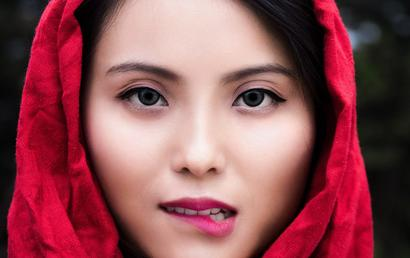
\includegraphics[width=.5\textwidth]{Chapters/03_SimpleML/4_kmeans/girl3.jpg}
    }
\end{figure}
% ******************************************************************************


% <div class="imgcap">
% <img src ="/assets/kmeans/girl3.jpg" align = "centroid">
% <div class="thecap">Credit ảnh: <a href = "https://www.facebook.com/photo.php?fbid=1219980151402370&set=a.113129725420757.13101.100001711890571&type=3&theater"> Trọng Vũ</a>
% </div>
% </div>


% \subsection{Lên ý tưởng  }
% (\textit{Lại giả sử rằng chúng ta chưa biết gì khác ngoài K-means clustering,
% các bạn hãy dừng vài giây để nghĩ xem chúng ta có thể xử lý thế nào. Gợi ý: Có
% ba màu chủ đạo trong bức ảnh.})

% Ok, có ba màu, ba clusters!

Bức ảnh có ba màu chủ đạo: hồng ở khăn và môi; đen ở mắt, tóc, và hậu cảnh; màu
da ở vùng còn lại của khuôn mặt. Ảnh này khá rõ nét và các vùng được phân biệt
rõ ràng bởi màu sắc nên chúng ta có thể áp dụng thuật toán phân cụm $K$-means.
Thuật toán này sẽ phân các điểm ảnh thành ba cụm, cụm chứa phần khuôn mặt có thể được chọn tự động hoặc bằng tay. 

Đây là một bức ảnh màu, mỗi điểm ảnh được biểu diễn bởi ba giá trị tương ứng với
màu đỏ, lục, và lam (RGB). Nếu coi mỗi điểm ảnh là một điểm dữ liệu được mô tả
bởi một vector ba chiều chứa các giá trị này, sau đó áp dụng phân cụm $K$-means,
chúng ta có thể đạt được kết quả như mong muốn.



\subsection{Làm việc trên Python}

{Khai báo thư viện và hiển thị bức ảnh:}

\begin{lstlisting}[language=Python]
import matplotlib.image as mpimg
import matplotlib.pyplot as plt
import numpy as np
from sklearn.cluster import KMeans
img = mpimg.imread('girl3.jpg')
plt.imshow(img)
imgplot = plt.imshow(img)
plt.axis('off')
plt.show()
\end{lstlisting}


{Biến đổi bức ảnh thành một ma trận mà mỗi hàng là ba giá trị màu của một điểm ảnh:}
\begin{lstlisting}[language=Python]
X = img.reshape((img.shape[0]*img.shape[1], img.shape[2]))
\end{lstlisting}

Phần còn lại của mã nguồn có thể được tìm thấy tại \url{https://goo.gl/Tn6Gec}.


% <div class="imgcap">
% <img src ="/assets/kmeans/girl_seg.png" align = "centroid">
% </div>

\begin{figure}[t]
    % caption on side     
    \floatbox[{\capbeside\thisfloatsetup{capbesideposition={right,top},capbesidewidth=6cm}}]{figure}[\FBwidth]
    {\caption{ 
    Kết quả nhận được sau khi thực hiện phân cụm $K$-means.
    Có ba cụm tương ứng với ba màu đỏ, hồng, đen (xem ảnh màu trong Hình~\ref{fig:5_girl_seg_c}). 
    }
    \label{fig:5_girl_seg}}
    { % figure here
    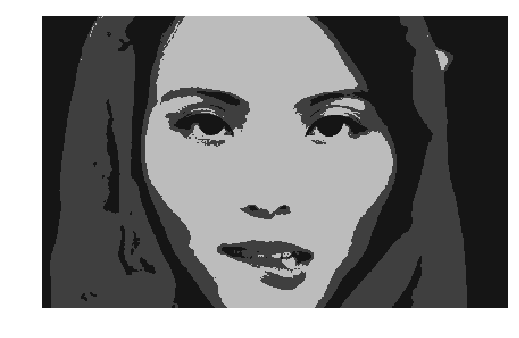
\includegraphics[width=.5\textwidth]{Chapters/03_SimpleML/4_kmeans/girl_seg_gray.png}
    }
\end{figure}

Sau khi tìm được các cụm, giá trị của mỗi pixel được thay bằng giá trị của
tâm tương ứng. Kết quả được minh hoạ trên Hình~\ref{fig:5_girl_seg}. Ba màu
đỏ, đen, và màu da (xem ảnh màu trong Hình~\ref{fig:5_girl_seg_c}) đã được phân
nhóm khá thành công. Khuôn mặt có thể được tách ra từ phần có màu da và vùng
bên trong nó. Như vậy, phân cụm $K$-means tạo ra một kết quả chấp nhận được
cho bài toán này.


\section{Nén ảnh}

Trước hết, xét đoạn code dưới đây:

\begin{lstlisting}[language=Python]
for K in [5, 10, 15, 20]:
    kmeans = KMeans(n_clusters=K).fit(X)
    label = kmeans.predict(X)

    img4 = np.zeros_like(X)
    # replace each pixel by its centroid
    for k in range(K):
        img4[label == k] = kmeans.cluster_centroids_[k]
    # reshape and display output image
    img5 = img4.reshape((img.shape[0], img.shape[1], img.shape[2]))
    plt.imshow(img5, interpolation='nearest')
    plt.axis('off')
    plt.show()
\end{lstlisting}

Nhận thấy rằng mỗi điểm ảnh có thể nhận một trong số $256^3 \approx $ 16 triệu
màu. Đây là một số rất lớn (tương đương với 24 bit cho một điểm ảnh). Phân cụm
$K$-means có thể được áp dụng để nén ảnh với số bit ít hơn. Phép nén ảnh này làm
mất dữ liệu nhưng kết quả vẫn chấp nhận được. Quay trở lại bài toán tách vật thể
trong mục trước, nếu thay mỗi điểm ảnh bằng tâm cụm tương ứng, ta thu được một
bức ảnh nén. Tuy nhiên, chất lượng bức ảnh rõ ràng đã giảm đi nhiều. Trong đoạn
code trên đây, ta đã làm một thí nghiệm nhỏ với số lượng cụm tăng lên 5, 10, 15,
20. Sau khi tìm được tâm cho mỗi cụm, giá trị của một điểm ảnh được thay bằng
giá trị của tâm tương ứng. Kết quả được hiển thị trên Hình~\ref{fig:5_res}. Có
thể thấy rằng khi số lượng cụm tăng lên, chất lượng bức ảnh đã được cải thiện.
Để nén bức ảnh này, ta chỉ cần lưu $K$ tâm cụm tìm được và nhãn của mỗi điểm
ảnh.



\begin{figure}[t]
\centering
    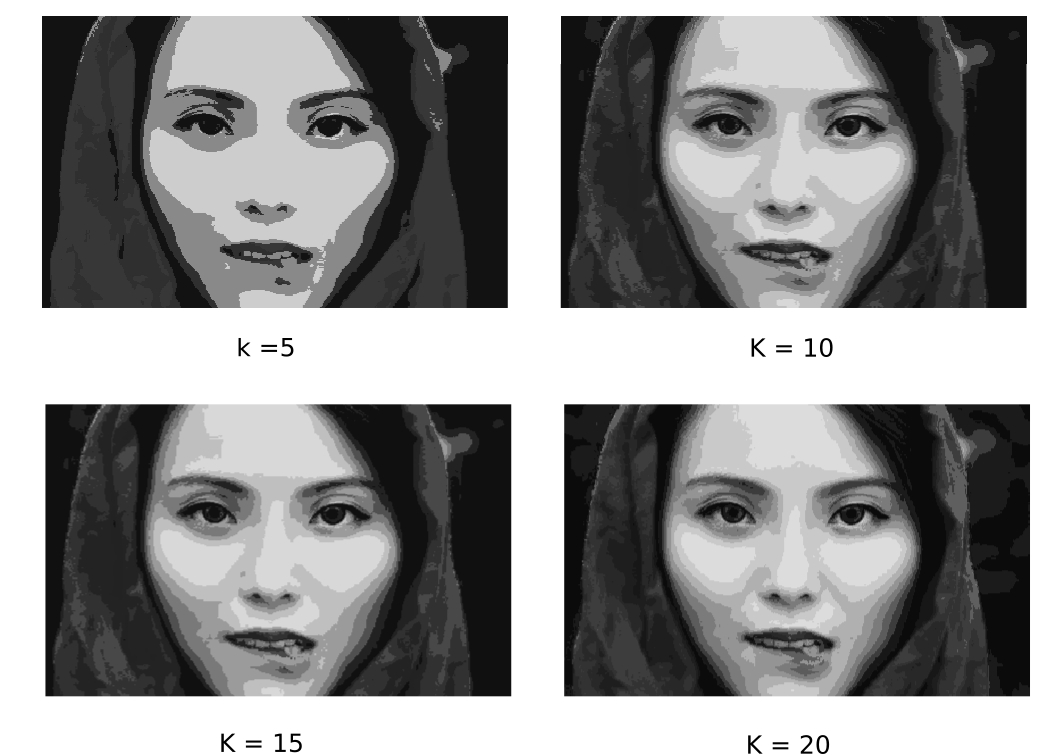
\includegraphics[width = \textwidth]{Chapters/03_SimpleML/4_kmeans/girl_all_gray.png}
    \caption[]{Chất lượng nén ảnh với số lượng cluster khác nhau (xem ảnh màu trong Hình~\ref{fig:5_res_c}).}
    \label{fig:5_res}
\end{figure}


\section{Thảo luận}
\subsection{Hạn chế của phân cụm $K$-means}


% \subsection{Hạn chế}
\index{phương pháp elbow}
% Có một vài hạn chế của thuật toán phân cụm $K$-means:
\begin{itemize}
    \item \textit{Số cụm $K$ cần được xác định trước.}
    Trong trường hợp, chúng ta không biết trước giá trị này. Bạn đọc có thể tham khảo \textit{phương pháp elbow} giúp xác định giá trị $K$ này (\url{https://goo.gl/euYhpK}).
% ******************************************************************************
    \begin{figure}[t]
        \begin{subfigure}{0.325\textwidth}
        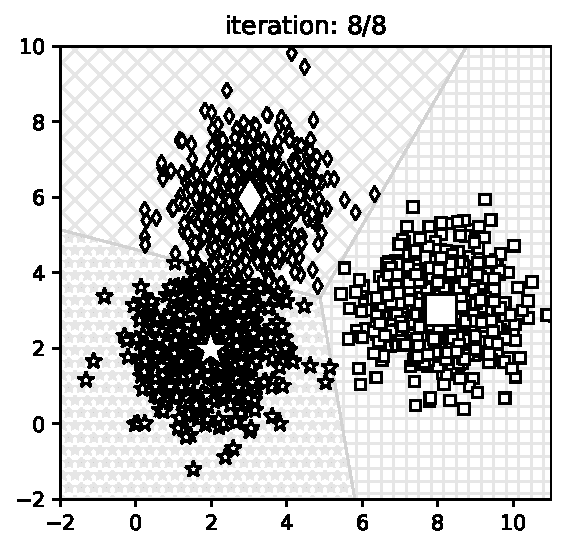
\includegraphics[width=0.99\linewidth]{ebookML_src/src/kmeans/dif_res10.pdf}
        \caption{}
        \label{fig:4_dif_resa}
        \end{subfigure}
        \begin{subfigure}{0.325\textwidth}
        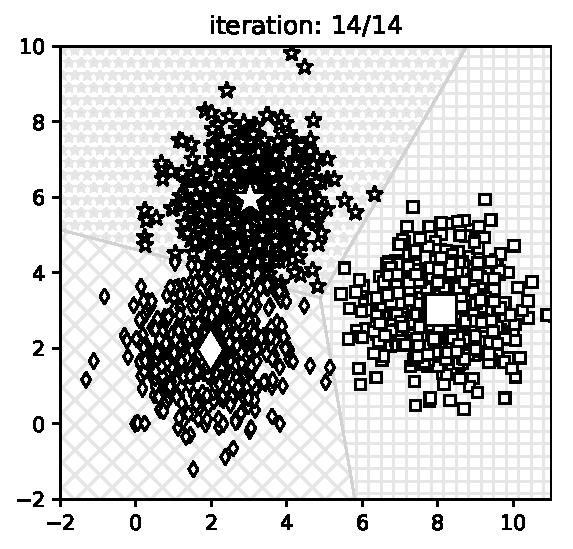
\includegraphics[width=0.99\linewidth]{ebookML_src/src/kmeans/dif_res31.pdf}
        \caption{}
        \label{fig:4_dif_resb}
        \end{subfigure}
        \begin{subfigure}{0.325\textwidth}
        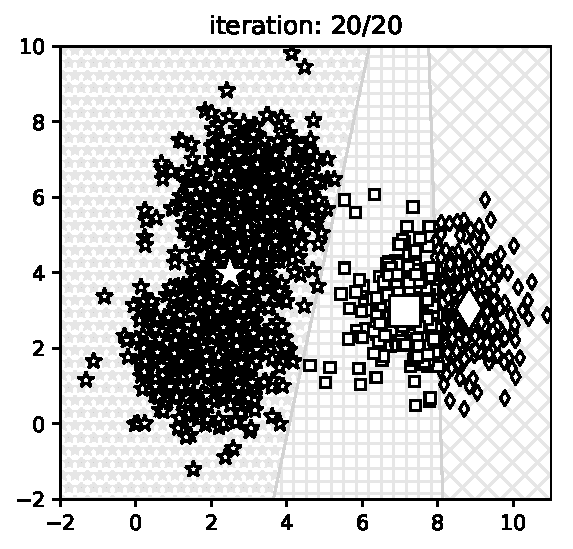
\includegraphics[width=0.99\linewidth]{ebookML_src/src/kmeans/dif_res27.pdf}
        \caption{}
        \label{fig:4_dif_resc}
        \end{subfigure}
        \caption{
        Các giá trị khởi tạo ban đầu khác nhau dẫn đến các nghiệm khác nhau. 
        }
        \label{fig:4_dif_res}
    \end{figure}
% ******************************************************************************
    \item \textit{Nghiệm cuối cùng phụ thuộc vào các tâm cụm được khởi tạo ban
    đầu.}
    Thuật toán phân cụm $K$-means không đảm bảo tìm được nghiệm tối ưu toàn cục, nghiệm cuối cùng phụ thuộc vào các tâm cụm được khởi tạo ban đầu.
    Hình~\ref{fig:4_dif_res} thể hiện các kết quả khác nhau khi các tâm cụm
    được khởi tạo khác nhau. Ta cũng thấy rằng trường hợp (a) và (b) cho kết quả
    tốt, trong khi kết quả thu được ở trường hợp (c) không thực sự tốt. Một điểm
    nữa có thể rút ra là số lượng vòng lặp tới khi thuật toán hội tụ cũng khác
    nhau. Trường hợp (a) và (b) cùng cho kết quả tốt nhưng (b) chạy trong thời
    gian gần gấp đôi. Một kỹ thuật giúp hạn chế nghiệm xấu như trường hợp (c) là
    chạy thuật toán phân cụm $K$-means nhiều lần với các tâm cụm được khởi tạo
    khác nhau và chọn ra lần chạy cho giá trị hàm mất mát thấp nhất\footnote{\textit{KMeans -- scikit-learn} (\url{https://goo.gl/5KavVn}).}. Ngoài ra, có một vài thuật toán giúp chọn các tâm cụm ban đầu~\cite{khan2004cluster},
    Kmeans++~\cite{arthur2007k,bahmani2012scalable}.
  
    \item \textit{Các cụm cần có số lượng điểm gần bằng nhau}.
    Hình~\ref{fig:4_disa} minh hoạ kết quả khi các cụm có số điểm
    chênh lệch. Trong trường hợp này, nhiều điểm lẽ ra thuộc cụm hình vuông đã bị phân nhầm vào cụm hình sao. 

    \index{Gaussion mixture model}
    \item \textit{Các cụm cần có dạng hình tròn (cầu)}.
    Khi các cụm vẫn tuân theo phân phối chuẩn nhưng ma trận hiệp phương sai
    không tỉ lệ với ma trận đơn vị, các cụm sẽ không có dạng tròn
    (hoặc cầu trong không gian nhiều chiều). Khi đó, phân cụm $K$-means không hoạt động hiệu quả. Lý do chính là vì phân cụm $K$-means quyết định
    nhãn của một điểm dữ liệu dựa trên khoảng cách Euclid của nó tới các
    tâm. Trong trường hợp này, \textit{Gaussian mixture models} (GMM)~\cite{reynolds2015gaussian} có thể cho kết quả tốt hơn\footnote{Đọc thêm:
    \textit{Gaussian mixture models -- Wikipedia} (\url{https://goo.gl/GzdauR}).}. Trong GMM, mỗi cụm được giả sử tuân theo một phân phối chuẩn với ma trận hiệp phương sai không nhất thiết tỉ lệ với ma trận đơn vị. Ngoài các tâm cụm, các ma trận hiệp phương sai cũng là các biến cần tối ưu trong GMM. 
    

    \index{phân cụm spectral -- spectral clustering}
    \item \textit{Khi một cụm nằm trong cụm khác}.
    Hình~\ref{fig:4_face} là một ví dụ kinh điển về việc phân cụm $K$-means
    không làm việc. Một cách tự nhiên, chúng ta sẽ phân dữ liệu ra thành bốn
    cụm: mắt trái, mắt phải, miệng, xung quanh mặt. Nhưng vì mắt và miệng nằm
    trong khuôn mặt nên phân cụm $K$-means cho kết quả không chính xác. Với dữ
    liệu như trong ví dụ này, \textit{phân cụm
    spectral}~\cite{von2007tutorial,ng2002spectral} sẽ cho kết quả tốt hơn. Phân
    cụm spectral cũng coi các điểm gần nhau tạo thành một cụm, nhưng không giả
    sử về một tâm chung cho cả cụm. Phân cụm spectral được thực hiện dựa trên
    một đồ thị vô hướng với đỉnh là các điểm dữ liệu và cạnh được nối giữa các
    điểm gần nhau, mỗi cạnh được đánh trọng số là một hàm của khoảng cách giữa
    hai điểm.
  

\end{itemize}


% ******************************************************************************
\begin{figure}[t]
    \begin{subfigure}{0.49\textwidth}
   
    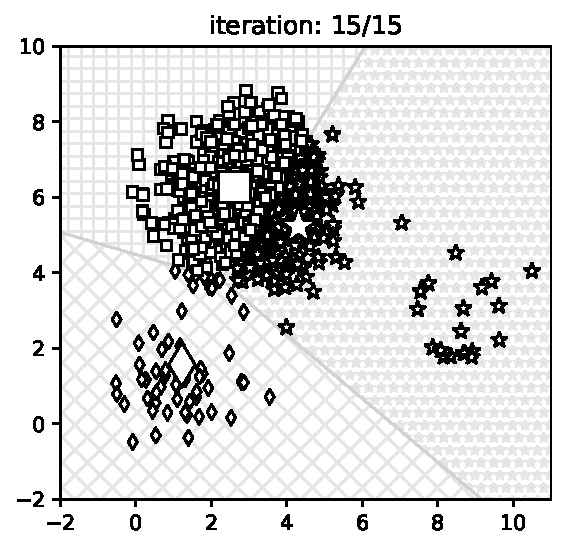
\includegraphics[width=0.8\linewidth]{ebookML_src/src/kmeans/skew_10.pdf}
    \caption{}
    \label{fig:4_disa}
    \end{subfigure}
    \begin{subfigure}{0.49\textwidth}
   
    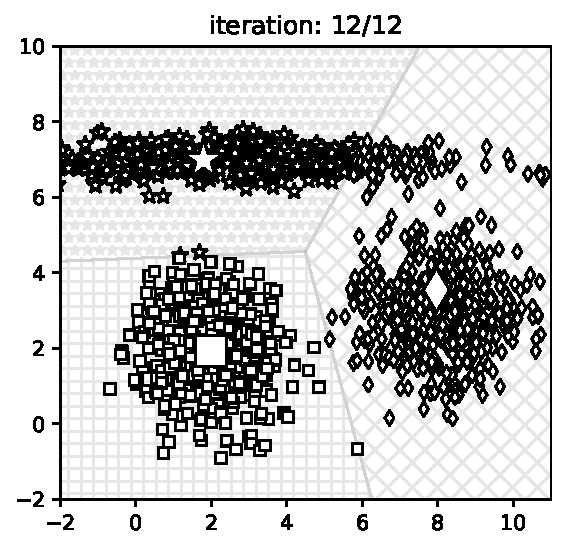
\includegraphics[width=0.8\linewidth]{ebookML_src/src/kmeans/notround_10.pdf}
    \caption{}
    \label{fig:4_disb}
    \end{subfigure}
    \caption{
     Phân cụm $K$-means hoạt động không thực sự tốt trong trường hợp các
     cụm có số lượng phần tử chênh lệch hoặc các cụm không có dạng
     hình tròn. 
    }
    \label{fig:4_dis}
\end{figure}
% ******************************************************************************



\begin{figure}[t]
    % caption on side     
    \floatbox[{\capbeside\thisfloatsetup{capbesideposition={right,top},capbesidewidth=6.5cm}}]{figure}[\FBwidth]
    {\caption{ 
        Một ví dụ về việc phân cụm $K$-means không hoạt động hiệu quả.
    }
    \label{fig:4_face}}
    { % figure here
    % 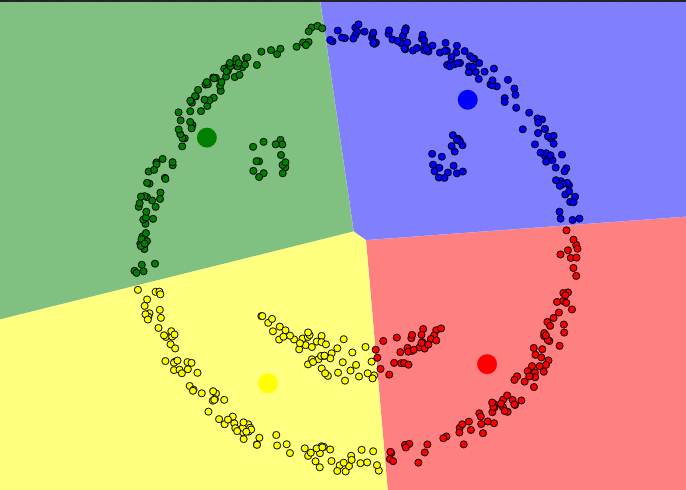
\includegraphics[width=.55\textwidth]{Chapters/03_SimpleML/4_kmeans/smile_face.png}
    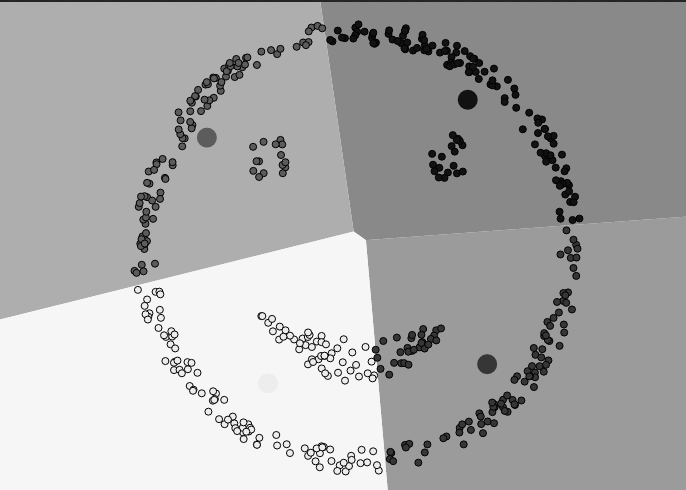
\includegraphics[width=.3\textwidth]{Chapters/03_SimpleML/4_kmeans/smile_face_gray.png}
    }
\end{figure}

\subsection{Các ứng dụng khác của phân cụm $K$-means}
Mặc dù có những hạn chế, phân cụm $K$-means vẫn cực kỳ quan trọng trong machine
learning và là nền tảng cho nhiều thuật toán phức tạp khác. Dưới đây là một vài ứng dụng khác của phân cụm $K$-means. 
% \begin{enumerate}
	% \item Với một thuật toán K-means clustering đơn giản, chúng ta đã có thể áp
	% dụng nó vào các bài toán thực tế. Mặc dù kết quả chưa thực sự như ý, chúng ta
	% vẫn thấy được tiềm năng của thuật toán đơn giản này.

    Cách thay một điểm dữ liệu bằng tâm cụm tương ứng là một trong số các
    kỹ thuật có tên chung là \textit{vector quantization  --
    VQ}~\cite{arya1993algorithms}). Không chỉ được áp dụng trong nén dữ liệu, VQ
    còn được kết hợp với Bag-of-Words\cite{lazebnik2006beyond} áp dụng rộng rãi
    trong các thuật toán xây dựng vector đặc trưng.


    Ngoài ra, VQ cũng được áp dụng vào các bài toán tìm kiếm trong cơ sở dữ liệu
    lớn. Khi số điểm dữ liệu là rất lớn, việc tìm kiếm trở nên cực kỳ quan
    trọng. Khó khăn chính của việc này là làm thế nào có thể tìm kiếm một cách
    nhanh chóng trong lượng dữ liệu khổng lồ đó. Ý tưởng cơ bản là sử dụng các
    thuật toán phân cụm để phân các điểm dữ liệu thành nhiều cụm nhỏ. Để tìm các
    điểm gần nhất của một điểm \textit{truy vấn}, ta có thể tính khoảng cách
    giữa điểm này và các tâm cụm thay vì toàn bộ các
    điểm trong cơ sở dữ liệu. Bạn đọc có thể đọc thêm các bài báo nổi tiếng gần
    đây về vấn đề này: Product Quantization~\cite{jegou2011product}, Cartesian
    k-means~\cite{norouzi2013cartesian,johnson2017billion}, Composite
    Quantization~\cite{zhang2014composite}, Additive
    Quantization~\cite{babenko2014additive}.


% \end{enumerate}
Mã nguồn cho chương này có thể được tìm thấy tại \url{https://goo.gl/QgW5f2}. 



\subsection{Đọc thêm}

\begin{enumerate}
	\item \textit{Clustering documents using k-means -- scikit-learn} (\url{https://goo.gl/y4xsy2}).

	\item \textit{Voronoi Diagram -- Wikipedia} (\url{https://goo.gl/v8WQEv}).

	\item \textit{Cluster centroid initialization algorithm for K-means clustering} (\url{https://goo.gl/hBdody}). 

	\item \textit{Visualizing K-Means Clustering} (\url{https://goo.gl/ULbpUM}). 

	\item \textit{Visualizing K-Means Clustering -- Standford} (\url{https://goo.gl/idzR2i}). 

\end{enumerate}

